\section{Formulación de problemas como programas lineales}

A parte de los ejemplos de la sección anterior que representan los problemas típicos de la programación lineal, podemos adaptar otro tipo de problemas para tratar de resolverlos mediante \textit{método Símplex} o similares.\\

Algunos de estos problemas son problemas de grafos, como el \textit{problema de flujo de mínimo coste en una red}; el \textit{problema de la mochila} o el \textit{problema de la dieta}.

\subsection{Problema de la dieta}
\begin{defi} Definimos el problema de la dieta como uno del siguiente tipo:

Se conocen los contenidos nutritivos de ciertos alimentos, sus precios y la cantidad mínima diaria de nutrientes aconsejada. Se denota por $m$ el número de nutrientes y por $n$ el número de alimentos considerados. La cantidad mínima del nutriente $i$ aconsejada es $b_i$, el precio de una unidad del alimento $j$ es $c_j$ y la cantidad de nutriente $i$ en una unidad del alimento $j$ es $a_{ij}$. El problema consiste en determinar la cantidad $x_j$, de cada alimento $j$, que debe comprarse de forma que se satisfagan los mínimos aconsejados y se alcance un precio total mínimo.
\end{defi}

\begin{ejem} Se considera un problema de la dieta con cinco alimentos y con los mínimos aconsejados para los nutrientes digeribles (DN), proteínas digeribles (DP), calcio (Ca) y fósforo (Ph), dados en la siguiente tabla.
\begin{center}
\begin{tabular}{|c|c|c|c|c|c|c|}
\hline
Nutriente & Cantidad requerida & Maíz A & Avena & Maíz B & Salvado & Linaza \\ \hline
DN & 74.2 & 78.6 & 70.1 & 80.1 & 67.2 & 77.0\\ \hline
DP & 14.7 & 6.50 & 9.40 & 8.80 & 13.7 & 30.4\\ \hline
Ca & 0.14 & 0.02 & 0.09 & 0.03 & 0.14 & 0.41\\ \hline
Ph & 0.55 & 0.27 & 0.34 & 0.30 & 1.29 & 0.56 \\ \hline
\end{tabular}
\end{center}
Los precios unitarios de los alimentos (en determinada unidad monetaria) son los siguientes:
\begin{center}
\begin{tabular}{|c|c|c|c|c|c|}
\hline
Alimento & Maíz A & Avena & Maíz B & Salvado & Linaza \\ \hline
Coste & 1 & 0.5 & 2 & 1.2 & 3\\ \hline
\end{tabular}
\end{center}
Procedamos a formular el problema, si nos fijamos, podemos lograr un problema del tipo de la \textit{definición 1.1}.\\

Identifiquemos nuestros datos: Tenemos $x_1$ como cantidad de Maíz A, $x_2$ como avena, $x_3$ como maíz B, $x_4$ como salvado y $x_5$ como linaza. Nuestra matriz de coeficientes de costos es $C=\begin{pmatrix}1\\0.5\\2\\1.2\\3\end{pmatrix}$. Por último, nuestra matriz de restricciones es\\
$\big(a_{ij}\big)\underset{1\leq i\leq 4}{\underset{1\leq j \leq 5}{\ }}=\begin{pmatrix}78.6 & 70.1 & 80.1 & 67.2 & 77.0\\6.50 & 9.40 & 8.80 & 13.7 & 30.4\\0.02 & 0.09 & 0.03 & 0.14 & 0.41\\0.27 & 0.34 & 0.30 & 1.29 & 0.56 \\\end{pmatrix}$ con $B=\begin{pmatrix}74.2\\14.7\\0.14\\0.55\end{pmatrix}$.\\

Es evidente que nuestro fin es reducir los costes de la compra de alimentos, luego nuestra función objetivo queda:
\[\min\ z = \stackbin[j=1]{5}\sum c_jx_j=x_1+0.5x_2+2x_3+1.2x_4+3x_5\]
Mientras que las restricciones surgen al tener que cumplir un requisito de nutrientes:
\[AX\geq B\equiv\left. \begin{array}{ll}	
 78.6x_1+70.1x_2+80.1x_3+67.2x_4+77.0x_5 \geq 74.2\\
 6.50x_1+9.40x_2+8.80x_3+13.7x_4+30.4x_5\geq 14.7\\
 0.02x_1+0.09x_2+0.03x_3+0.14x_4+0.41x_5\geq 0.14\\
 0.27x_1+0.34x_2+0.30x_3+1.29x_4+0.56x_5\geq 0.55\\	 \end{array} \right.\]
\[x_1,x_2,x_3,x_4,x_5\geq 0\]

Luego el problema es resoluble por el mismo método que lo eran los ejemplos de la sección anterior, mediante la búsqueda del vértice de menor coste de la región factible originada en $\R^5$, es decir, mediante el \textit{método Símplex}.

La solución lineal de este problema es:
\[x_1= 0,x_2 = \dfrac{2857}{1867}, x_3 = 0, x_4 = \dfrac{43}{1867}, x_5 = 0\ \mathrm{con\ }z = \dfrac{12801}{18670}.\]

Cabe la pena destacar que el enunciado podría restringir a cantidades enteras la compra de alimentos, haciendo que nuestra solución fuera incorrecta. Este tipo de restricciones no son objeto de estudio de la programación lineal, sino que lo son de la programación entera que no trataremos en este texto.
\end{ejem}

\subsection{Problema del transporte}
\begin{defi} Definimos el problema del transporte como uno del siguiente tipo:

Un determinado producto debe enviarse en cantidades especificadas $a_1,… ,a_m$ desde $m$ centros de suministro y recibirse en cantidades especificadas $b_1,…,b_n$, en $n$ centros de demanda. El coste del envío de una unidad de producto desde el origen $i$ al destino $j$ es $c_{ij}$. El problema consiste en determinar las cantidades $x_{ij}$, que deben enviarse desde el origen $i$ al destino $j$, para conseguir minimizar el coste del envío.
\end{defi}

\begin{ejem} En este caso, en lugar de ver un caso concreto, formulemos las condiciones anteriores.\\

Nuestra función objetivo es la suma de costes de las cantidades enviadas; es decir:
\[\min z=\stackbin[i=1]{m}\sum\stackbin[j=1]{n}\sum c_{ij}x_{ij}\]
Por lo que nuestra solución es un vector de la región factible del problema originada en $\R^{m\cdot n}$.

En cuanto a las restricciones, se limitan a cumplir las solicitudes de los centros de demanda, luego tenemos $n$ restricciones del tipo:
\[\stackbin[i=1]{m}\sum a_ix_{ij}\geq b_j\ \ \forall 1\leq j\leq n\]

Por supuesto, y como siempre, concluimos con que $x_{ij}\geq 0$ $\ \forall 1\leq i\leq m,\ \ \forall 1\leq j\leq n$.
\end{ejem}

\subsection{Problema de flujo de mínimo coste en una red}
\begin{defi} Definimos el problema del flujo mínimo en una red como uno del siguiente tipo:

Se considera una red de transporte (por ejemplo de transporte de locomoción, un sistema de comunicaciones, etcétera) a través de la cual se desea enviar un determinado producto desde ciertos puntos de la red, llamados nodos fuente, hasta otros puntos de destino, llamados sumideros. Además de estas dos clases de nodos, la red puede contener nodos intermedios, donde no se genera ni se consume el producto que está fluyendo por la red. Se denota por $b_i$, el suministro del nodo $i$ (si $i$ es un nodo fuente) y por $-b_i$, la demanda del nodo $i$ (si $i$ es un nodo sumidero). Se denota por $x_{ij}$, el flujo que se envía desde el nodo $i$ al nodo $j$; $u_{ij}$, la capacidad máxima de flujo en la conexión entre el nodo $i$ y el nodo $j$ y por $c_{ij}$, el precio de enviar una unidad del producto desde el nodo $i$ y al nodo $j$. El problema consiste en determinar las cantidades $x_{ij}$, que deben enviarse, para conseguir minimizar el coste total de los envíos.
\end{defi}

\begin{ejem} Veamos un ejemplo de problema flujo mínimo en una red:\\

Se considera el problema de hallar un flujo de mínimo coste en la red con capacidades de la \textit{figura 3.1}, donde cada arco indica su coste y su capacidad ($c_{ij}$, $u_{ij}$). Se considera un único vértice fuente (el vértice 1, con suministro de 20 unidades) y un único vértice sumidero (el vértice 6, con demanda de 20 unidades).\newpage

\begin{figura}\ \begin{center}\definecolor{zzttqq}{rgb}{0.15,0.35,0.15}

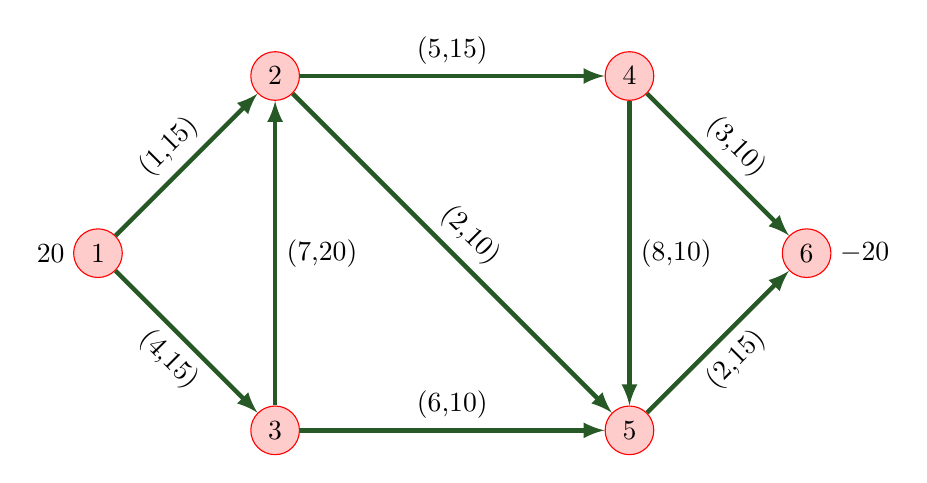
\begin{tikzpicture}[x=1.5cm, y=1.5cm]
	\fill (-3.2,0) circle (0.1pt)node[anchor=east] {$20$};
	\fill (3.2,0) circle (0.1pt)node[anchor=west] {$-20$};
    \node[circle,draw=red,fill=red!20!] (v2) at (-1.5,1.5) {2};
    \node[circle,draw=red,fill=red!20!] (v4) at (1.5,1.5) {4};
    \node[circle,draw=red,fill=red!20!] (v6) at (3,0) {6};
    \node[circle,draw=red,fill=red!20!] (v5) at (1.5,-1.5) {5};
    \node[circle,draw=red,fill=red!20!] (v3) at (-1.5,-1.5) {3};
    \node[circle,draw=red,fill=red!20] (v1) at (-3,0) {1};
    \draw[color=zzttqq, ultra thick, -latex]  (v1) edge node[rotate = 45, above,color=black]{(1,15)} (v2);
	\draw[color=zzttqq, ultra thick, -latex]  (v1) edge node[rotate = -45, below,color=black]{(4,15)} (v3);
	\draw[-latex, color=zzttqq, ultra thick]  (v3) edge node[right,color=black]{(7,20)} (v2);
	\draw[-latex, color=zzttqq, ultra thick]  (v2) edge node[above,color=black]{(5,15)} (v4);
	\draw[-latex, color=zzttqq, ultra thick]  (v3) edge node[above,color=black]{(6,10)} (v5);
	\draw[-latex, color=zzttqq, ultra thick]  (v2) edge node[rotate=-45,above,color=black]{(2,10)} (v5);
	\draw[-latex, color=zzttqq, ultra thick]  (v4) edge node[right,color=black]{(8,10)} (v5);
	\draw[-latex, color=zzttqq, ultra thick]  (v4) edge node[rotate=-45,above,color=black]{(3,10)} (v6);
	\draw[-latex, color=zzttqq, ultra thick]  (v5) edge node[rotate=45,below,color=black]{(2,15)} (v6);
    \end{tikzpicture}\end{center}\end{figura}

Planteemos nuestra función obejtivo. Recordemos que hemos definido $x_{ij}$ como la cantidad llevada del nodo $i$ al $j$ y $c_{ij}$ el coste por unidad transportada de $i$ a $j$, luego nuestra función objetivo es:
\[\min z=\stackbin[i=1]{m}\sum\stackbin[j=1]{n}\sum c_{ij}x_{ij}\] En este caso podemos expresar de forma más concreta la función anterior, pues en realidad sólo tenemos 9 aristas:
\[\min z=c_{12}x_{12}+c_{13}x_{13}+c_{24}x_{24}+c_{25}x_{25}+c_{32}x_{32}+c_{35}x_{35}+c_{45}x_{45}+c_{46}x_{46}+c_{56}x_{56}=\]
\[=x_{12}+4x_{13}+5x_{24}+2x_{25}+7x_{32}+6x_{35}+8x_{45}+3x_{46}+2x_{56}\]

Hablemos ahora de las restricciones. Si un vértice $i$ es intermedio, la cantidad de producto y recibida es la misma, luego denotamos $b(i)=0$. Es decir, se debe cumplir que\\
$\stackbin[j=1]{6}\sum x_{ij}-\stackbin[j=1]{6}\sum x_{ji}=0$. Y para los vértices fuente y sumidero (1 y 6 respectivamente) se tiene que cumplir que $\stackbin[j=1]{6}\sum x_{ij}-\stackbin[j=1]{6}\sum x_{ji}=20$ y $\stackbin[j=1]{6}\sum x_{ij}-\stackbin[i=1]{6}\sum x_{ji}=-20$ respectivamente. Luego estas restricciones pueden ser representadas de forma matricial de la siguiente forma:
\[\underset{A}{\underset{\shortparallel}{\begin{pmatrix}
1&1&0&0&0&0&0&0&0\\
-1&0&1&1&-1&0&0&0&0\\
0&-1&0&0&1&1&0&0&0\\
0&0&-1&0&0&0&1&1&0\\
0&0&0&-1&0&-1&-1&0&1\\
0&0&0&0&0&0&0&-1&-1
\end{pmatrix}}}\begin{pmatrix}x_{12}\\x_{13}\\x_{24}\\x_{25}\\x_{32}\\x_{35}\\x_{45}\\x_{46}\\x_{56}\end{pmatrix}=\begin{pmatrix}20\\0\\0\\0\\0\\-20\end{pmatrix}\]
\end{ejem}

Donde la matriz $A$ representa con cada una de sus 6 filas un vértice (la fila $i$-ésima representa el $i$-ésimo vértice) y cada una de sus 9 columnas representan una arista (en el orden que han sido escritas en la función objetivo). El valor 1 se corresponde con una arista que parte de ese vértice, y el -1 con una arista que llega al mismo (por lo que en cada columna hay un 1, un -1 y el resto ceros. Escribamos las ecuaciones resultantes de la igualdad matricial anterior:
\begin{align*} x_{12}+x_{13}=20\\-x_{12}+x_{24}+x_{25}-x_{32}=0\\-x_{13}+x_{32}+x_{35}=0\\-x_{24}+x_{45}+x_{46}=0\\-x_{25}-x_{35}-x_{45}+x_{56}=0\\-x_{46}-x_{56}=-20\end{align*}
Por último añadimos las últimas y no menos importantes:
\[0\leq x_{ij}\leq u_{ij}\ \ \mathrm{equivalentemente:}\]
\begin{align*} 0\leq x_{12}\leq 15,\ \ \ 0\leq x_{13}\leq 15,\ \ \ 0\leq x_{24}\leq 15,\\
0\leq x_{25}\leq 10,\ \ \ 0\leq x_{32}\leq 20,\ \ \ 0\leq x_{10}\leq 15,\\
0\leq x_{45}\leq 10,\ \ \ 0\leq x_{46}\leq 10,\ \ \ 0\leq x_{56}\leq 15
\end{align*}

Como podemos corroborar, hemos vuelto a conseguir un planteamiento lineal, al igual que en todos los ejemplos anteriores. Eso sí, esta vez hemos obtenido hasta 9 incógnitas y 15 restricciones, que señala que no siempre los problemas podrán ser resueltos cómodamente. Sin ir más lejos, región factible y solución de este problema se alojan en $\R^9$.\\

Por último señalar, como dato, que la solución del problema es $x_{12}=15\ ,x_{13}=5,\\x_{24}=5,\ x_{25}=10\ ,x_{32}=0\ ,x_{35}=5\ ,x_{45}=0\ ,x_{46}=5\ ,x_{56}=15$ con $z=155$.

\subsection{Problema de la mochila}

\begin{defi} Definimos el problema de la mochila como uno del siguiente tipo:

Se dispone de un presupuesto $b$ para invertir durante un determinado periodo de
tiempo, y se consideran $n$ proyectos. El proyecto $j$ requiere una inversión $a_j$ y proporciona
un beneficio $c_j$ . El objetivo es elegir un conjunto de proyectos de forma que no se exceda
el presupuesto y se obtenga el máximo beneficio.
\end{defi}

\newpage\begin{ejem} Veamos un ejemplo de problema de la mochila:\\

Sean 4 proyectos: el primero, de inversión $a_1=2$ y beneficio $c_1=10$; el segundo, con $a_2=1\y c_2=7$; el tercero, con $a_3=6$ y $c_3=25$ y el cuarto, $a_4=5$ y $c_4=24$. Además tenemos $b=7$ unidades para invertir. Calculemos el beneficio máximo sin exceder el presupuesto.

Podríamos formular el problema de la siguiente manera:
\[\max\ z = \stackbin[i=1]{4}\sum c_ix_i=10x_1+7x_2+25x_3+24x_4\]
como función objetivo y la restricción:
\[\stackbin[i=1]{4}\sum a_ix_i\leq b\equiv 2x_1+x_2+6x_3+5x_4\leq 7\]
Donde $x_i$ toma valor 0 si no escogemos el proyecto y 1 si es escogido; Es decir,\\
$x_i\in\{0,1\}\ \forall 1\leq i\leq 4$. Esta restricción nos convierte el problema en uno de programación entera. Veamos cómo resolver este tipo de problemas.

Definamos el problema:
\[f_r(\lambda)=\max\ \stackbin[i=1]{r}\sum c_ix_i\]
\[\mathrm{Sujeto\ a\ la\ restricc\acute{o}n\ }\stackbin[i=1]{r}\sum a_ix_i\leq\lambda\]
\[x_i\in\{0,1\}\ \forall 1\leq i\leq r\y\lambda\in\{1,...,b\}\]
Es claro que $z=f_n(b)$. Definimos \begin{align*} f_1(\lambda)&=0&\mathrm{\ si\ } 0\leq\lambda<a_1\\
f_1(\lambda)&=\max\{c_1,0\}&\mathrm{\ si\ } \lambda\geq a_1\\
f_r(\lambda)&=\max\{f_{r-1}(\lambda), c_r+f_{r-1}(\lambda-a_r)&\mathrm{\ en\ otro\ caso}
\end{align*}

Calculemos recursivamente $f_2,f_3\y f_4$ a partir de $f_1$ para todos los valores $\lambda=1,...,b$. Para identificar la solución óptima de $f_r(\lambda)$ utilizamos un indicador\\
$p_r(\lambda)=\doubleleft{0\mathrm{\ si\ }f_r(\lambda)=f_{r-1}(\lambda)}{1 \mathrm{\ en\ caso\ contrario}}$\\

En la siguiente tabla se muestran los distintos valores de $f_r(\lambda)$ y $p_r(\lambda)$:

\begin{center}\begin{tabular}{|c||c|c|c|c||c|c|c|c|}
\hline
$\lambda$&$f_1$&$f_2$ & $f_3$ & $f_4$ & $p_1$ & $p_2$ & $p_3$ & $p_4$ \\ \hline\hline
0 & 0  & 0  & 0  & 0  & 0 & 0 & 0 & 0\\ \hline
1 & 0  & 7  & 7  & 7  & 0 & 1 & 0 & 0\\ \hline
2 & 10 & 10 & 10 & 10 & 1 & 0 & 0 & 0\\ \hline
3 & 10 & 17 & 17 & 17 & 1 & 1 & 0 & 0\\ \hline
4 & 10 & 17 & 17 & 17 & 1 & 1 & 0 & 0\\ \hline
5 & 10 & 17 & 17 & 24 & 1 & 1 & 0 & 1\\ \hline
6 & 10 & 17 & 25 & 31 & 1 & 1 & 1 & 1\\ \hline
7 & 10 & 17 & 32 & 34 & 1 & 1 & 1 & 1\\ \hline
\end{tabular}\end{center}

La idea del algoritmo es comparar, a la hora de calcular $f_r(\lambda)$, si obtenemos un mejor resultado cogiendo o no $x_r$. Como $x_r$ tiene una inversión $a_r$, si es escogido, nos queda $\lambda-a_r$ presupuesto, por lo que miramos en la tabla el valor $f_{r-1}(\lambda-a_r)$. Si cogerlo es conveniente tenemos un nuevo máximo y apuntamos un 1 en $p_r(\lambda)$. Sobra decir que si la inversión de $x_r$ es mayor que $\lambda$ no podremos cogerlo en ningún caso.\\

Es interesante recalcar que el uso de programación dinámica para guardar los datos de la anterior tabla es altamente recomendable, puesto que nos ahorraremos numerosos cálculos recursivos ya hechos, quedando de esta manera una complejidad de $\mathcal{O}(bn)$.\\

Por último, falta que las $p_r(\lambda)$ guardadas jueguen su papel. Las hemos guardado porque sabemos que $\max\ z=f_4(7)=34$, pero desconocemos qué variables hemos tomado y cuáles no. Procedemos de la siguiente manera:\\

Empezamos por $p_4(7)$ que es 1, luego hemos tomado $x_4=1$ y esto implica que\\
$f_4(7)=f_3(7-a_4) +c_4\ximplies{p_3(2)=0}{}$ no hemos tomado $x_3$ y $f_3(2)=f_2(2)\ximplies{p_2(2)=0}{}$ no hemos tomado $x_2$ y $f_2(2)=f_1(2)\ximplies{p_1(2)=1}{}$ hemos tomado $x_1$. Luego $x_1=1,\ x_2=0,\ x_3=0,\ x_4=1\y z=34$.
\end{ejem}